\documentclass[10pt, conference, compsocconf]{IEEEtran}
\usepackage{color,graphicx}
\usepackage{amsmath}
\usepackage{amssymb}
%\usepackage{color}
%\usepackage{algorithm}
\usepackage[ruled]{algorithm2e}
%\usepackage{algorithmic}
\usepackage{enumerate}
%\usepackage{syntonly}
\usepackage{multicol}
\usepackage{multirow}
\usepackage{array}
%\usepackage[tight,footnotesize]{subfigure}https://www.overleaf.com/project/5cfd43d4b41ca5117%63f7621
%\usepackage{stfloats}
\usepackage{url}
\usepackage{threeparttable}
\usepackage{cite}
%\newtheorem{theorem}{Theorem}
%\newtheorem{lemma}{Lemma}
%\newtheorem{remark}{Remark}
\usepackage{svg}
\usepackage{nomencl}
\usepackage{tikz}
\usepackage{float}
\usepackage{etoolbox}
\makeatletter
\patchcmd{\@makecaption}
  {\scshape}
  {}
  {}
  {}
\makeatletter
\patchcmd{\@makecaption}
  {\\}
  {.\ }
  {}
  {}
\makeatother
\def\tablename{Table}

\usepackage{natbib}
\setlength{\bibsep}{1.0pt}
\newcolumntype{M}[1]{>{\centering\arraybackslash}m{#1}}

% End of preamble
%%%%%%%%%%%%%%%%%%%%%%%%%%%%%%%%%%%%%%%%%%%%%%%%%%%%%%%%%%%%%%%%%%%%%%%%%%%%%%%%%%%%%%%%

\author{ \parbox{5 in}{\centering Rohit Das\\
         Dept. of Electrical Engg. and Computer Science (EECS),\\
         Indian Institute of Technology, Bhilai\\
         Sejbahar, Chhattisgarh - 492015.\\
         {\tt\small rohitd@iitbhilai.ac.in}} % <-this % stops a space
}

%\IEEEoverridecommandlockouts
%\IEEEpubid{\makebox[\columnwidth]{978-1-4799-6016-3/14/\$31.00~\copyright~2014 IEEE \hfill} \hspace{\columnsep}\makebox[\columnwidth]{ }}

\begin{document}

\bstctlcite{IEEEexample:BSTcontrol}
\title{Generative Adversarial Network for Intrusion Detection Evasion}
\maketitle

\begin{abstract}

Intrusion Detection Systems (IDS) have been implemented using various Machine Learning models over the years. However, their robustness in the face of an adversary is something that has been lacking research. While current IDSs can detect between normal and malicious traffic, they may fail if a malicious traffic is disguised as normal. This paper aims to evade current IDSs by generating adversarial malicious traffic using a Wasserstein Generative Adversarial Network (WGAN) and hence test their robustness.The main idea here is that a black-box IDS will be used to classify half of the data set used (NSL-KDD) and the corresponding learning loss shall be recorded. Based on the predicted labels of the black-box IDS, the discriminator of IDSGAN will learn those labels and mimic the black-box to a certain extent. The predicted labels of the discriminator will then be fed back to the generator, which will accordingly learn and add noise to reduce its own loss of evading detection by the IDS.\\

The scope of the paper is limited by the dirth of data on attacks of the categories User2Root (U2R) and Remote2Local (R2L) in the data set NSL-KDD. Hence, further data collection in this area shall be a definite improvement for IDSGAN. Future improvements will be headed towards evasion in distributed computing, cloud computing and edge computing. Our research shall be specifically focused on how IDSGAN can be used to evade IDS for an Internet-of-Things (IoT) network. Such a network may be consisting of homogeneous edge-computing devices or heterogeneous devices like mobile phones, printers, etc., which may have their own IDS models built-in or a single distributed IDS model. Given the data for IDSGAN in evading various black-box models individually, we can create a distributed IDSGAN for the devices in the network and train according to the IDS being used. The IDSGAN will be specifically targeting any network-based intrusion detection system (NIDS) present in the network as it is mainly trained on network data, and not on system/host information, on which a host-based intrusion detection system (HIDS) is based.

\end{abstract}

% keywords can be removed
\begin{IEEEkeywords}
Deep learning, black box attack, adversarial learning, perturbation, intrusion detection.
\end{IEEEkeywords}


\section {Introduction}

With greater threats to security and robustness of networks comes greater responsibility on intrusion detection systems to detect and defend a network from malicious activities. The IDS monitors network traffic and raises alerts if it detects some kind of unauthorized and/or malicious activity. Its main aim is to classify between normal and malicious traffic.

Machine learning has been actively taking over that responsibility and has been shown to be performing quite well. Models based on learning algorithms like K-Nearest neighbours or Support Vector Machines have been utilized in IDSs and have achieved good results {\cite{tsai2009intrusion}}. Rapid developments in deep learning led to further improvements in IDSs like Convolutional Neural Networks (CNN), Recurrent Neural Networks, Auto-Encoders, etc \cite{li2017intrusion} \cite{li2018character}.

However, it was soon noticed that the IDSs werent't as robust under adversarial examples; inputs similar to the original data but misclassified due to some indistinguishable perturbation introduced in the dataset \cite{carlini2017adv}. With the introduction of GAN (generative adversarial networks) by Goodfellow \cite{goodfellow2014gan}, where a model contained two competing networks, generating adversarial data became much more convenient, and hence making systems more robust through adversarial training \cite{kim2017malware}. Although much work has been done in intrusion detection systems and GAN, here the paper highlights the use of GAN in IDS, thereby producing IDSGAN \cite{lin2018idsgan}. The main aim of IDSGAN is to use a black-box based on some generic learning algorithm, which will predict classes based on some initial adversarial data generated by the GAN generator. The discriminator will train itself based on the black-box output to mimic it as closely as possible. The predicted classes will then be fed back to the generator to train it and generate better adversarial models which can successfully evade an IDS with a high probability. The design and improvements in the generator and discriminator is done on the basis of Wasserstein GAN\cite{arjovsky2017gan} for its superior characteristics. To summarize, the following are contributed by this paper:

\begin{itemize}

\item The malicious data is modified so as not to invalidate its attack characteristic, i.e., only non-functional features are modified or removed.

\item To be as close to real-life situations and applications as possible, the adversarial attacks will be performed on black-box IDSs based on commonly-used Machine Learning models.

\item Experimentally, IDSGAN has shown to have successfully evaded all the black-box models used, meaning that most adversarial attacks went undetected by the IDSs used.

\item Improvements on the current IDSGAN, such as a distributed IDSGAN for distributed clusters, or IoT networks have also been discussed later in the paper.

\end{itemize}

\begin{figure*}

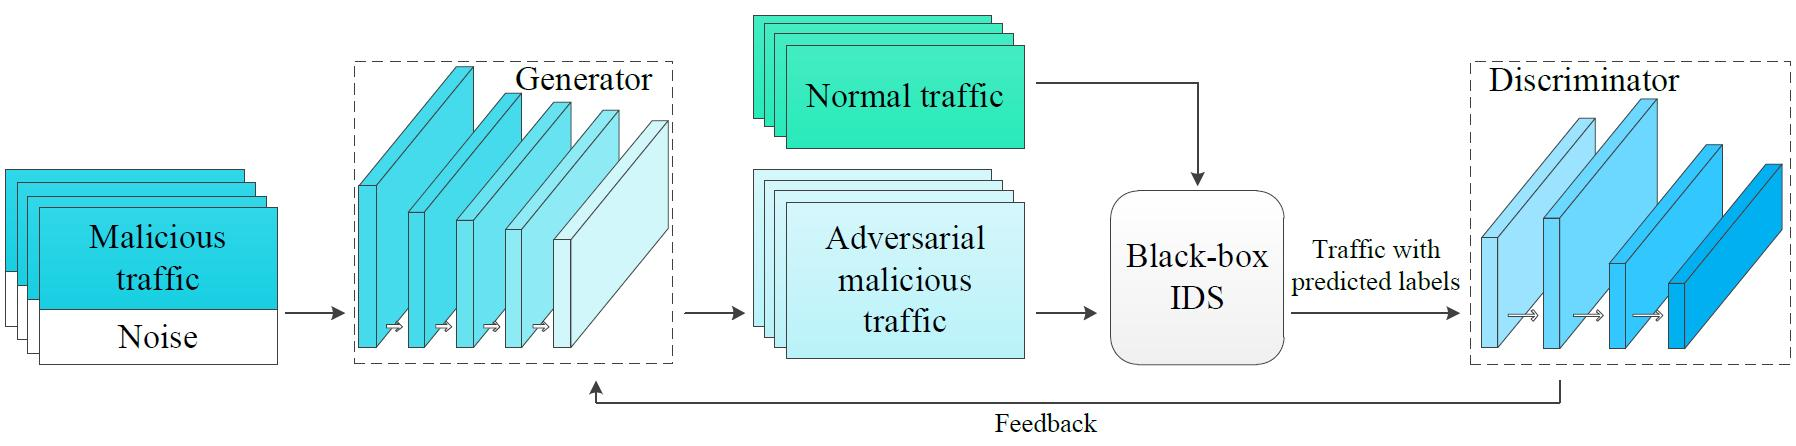
\includegraphics[width=\textwidth]{./images/img1.jpeg}
\caption{The training of IDSGAN. The training dataset is divided into the normal traffic and the malicious traffic. After adding
noise, the malicious traffic is sent into the generator. The adversarial malicious traffic and the normal traffic are predicted by the black-box IDS. The predicted labels and the original labels are used in the discriminator to simulate the black-box IDS. The
loss of generator is calculated based on the result of the discriminator and the predicted labels of the black-box IDS.}

\end{figure*}

\section {Problem Definition and Background }

The improved NSL-KDD is used as a benchmark and state-of-the-art dataset to evaluate any IDS \cite{hu2015improv}. The dataset is internally divided into the training set KDDTrain+ and the test set KDDTest+. To emulate real-world network traffic, the dataset consists of normal as well as 4 kinds of malicious traffic: Probing (Probe), Denial of Service (DoS), User2Root (U2R) and Root2Local (R2L). The features of the dataset can be broadly classified into four classes: "intrinsic", "content", "time-based traffic" and "host-based traffic" \cite{davis2011data} \cite{lee2000frame}. The detailed description is listed below:

\begin{itemize}

\item "Intrinsic" features: These features contain information about metadata obtained from packet headers.

\item "Content" features: These features hold actual information that is contained within packets.

\item "Time-based" traffic: These features hold data over analysis of traffic input over a 2-second window and contains information like how many connections were attempted to the same host.

\item "Host-based" traffic: These features store information about analysis over a series of connections made (how many requests made to the same host over x-number of connections). These features are designed to access attacks, which span longer than the 2-second window span.

\end{itemize}

All in all, the dataset contains 4 categorical, 6 binary, 23 discrete and 10 continuous features, totalling to 43. The last two features show the type of attack and score based on attack intensity.

For pre-processing of data, the values are put through numerical conversion and normalization to be converted to input vectors for traffic examples of IDSGAN. For the non-numeric discrete features, the distinct values are mapped to numbers. E.g., "protocol$\_$type" has 3 distinct values: TCP, UDP and ICMP. Each value can be assigned a discrete number like 1,2 and 3. In later stages, to eliminate the dimensional impact among feature values in input vectors, a standard scalar is used to normalize the original and converted numeric features into a specific range. Min-max normalization method is implemented to transform data within the interval $[0,1]$, thus suitable for all discrete and continuous features. The min-max normalization is calculated as follows:

\begin{center}

$x' = \dfrac{x - x_{min}}{x_{max} - x_{min}}$

\end{center}

$x$ being the feature value before normalization and $x'$ is the value after normalization. $x_{max}$ and $x_{min}$ represent the max and min value of this feature in the dataset respectively.

\section {Methodology and result}
Although rapid development in GANs has led to its many versions for many specific requests, it is instable and and causes non-convergence. To avoid such situations, Wasserstein GAN will be used for IDSGAN. In our model, the generator modifies specific features to produce adversarial malicious traffic data. A black-box IDS takes in the adversarial input, and predicts the classes. The discriminator takes the predicted labels of the black-box as input and tries to imitate it. The black-box IDS is implemented using some machine learning algorithm trained for intrusion detection. The framework of IDSGAN is represented in Fig. 1.

While we are generating malicious traffic data to evade the IDS, the attack capability of the data should be unaltered. So, it is evident that each category of attacks have some functional features which should not be changed. For the other non-functional attacks, we can choose to either keep or kick them. The functional features for each attack is highlighted in the table below \cite{lee2000frame}:

\begin{table}[ht]

\caption{The functional features of each attack category}

\begin{tabular}{*{5}{|M{4.8em}}|}
\hline
\multirow{2}{*}{Attack} & \multicolumn{4}{c|}{Functional features}                                                           \\[1.5ex] \cline{2-5}
 & Intrinsic & Content  & Time-based Traffic  & Host-based traffic \\[1.5ex] \hline
Probe &  \checkmark  &  & \checkmark & \checkmark\\[1.5ex] \hline
DoS & \checkmark   & & \checkmark  & \\[1.5ex] \hline
U2R & \checkmark  & \checkmark  &  & \\[1.5ex] \hline
R2L & \checkmark  &  \checkmark  &  &\\[1.5ex] \hline
\end{tabular}

\end{table}

\subsection{Results}

IDSGAN is trained with the 64 batch size for 100 epochs. The learning rates of the generator and the discriminator are both 0.0001. The dimension of the noise vector is 9. The weight clipping threshold for the discriminator training is set as 0.01. The experimental results have been performed with various black-box IDS models based on algorithms like Support Vector Machines (SVM), Multilayer Perceptrons (MLP), etc. The IDSGAN generates adversarial traffic which successfully evades all the black-box IDS models tested against it. A graphical representation of the results is shown in Fig. 2 \cite{lin2018idsgan}.

\begin{center}

\begin{figure}
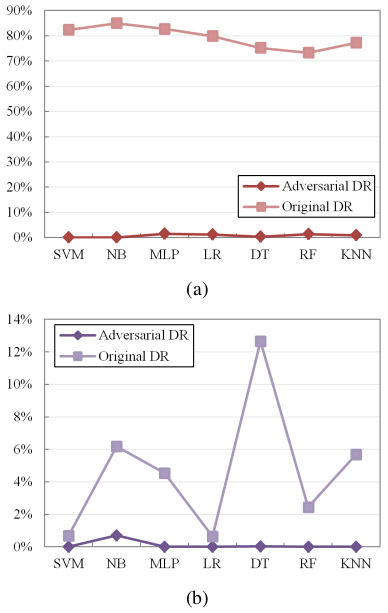
\includegraphics[width=0.47\textwidth]{./images/img2.png}
\caption{The comparisons of the adversarial detection rates and the original detection rates under different black-box IDS models with only the functional features unmodified. (a) is the results of DoS and (b) is results of U2R and R2L.}
\end{figure}

\end{center}

\section {Improvement Proposal}

While IDSGAN is seen to perform well for various black-box models, the research is mostly done for stand-alone devices like personal computers, connected to a network. An improvement for the current centralized IDSGAN would be a distributed network of generators, which can then be used to attack a distributed cluster system. The benefit of such a distributed GAN would be that each generator will be able to learn from its neighbouring devices, and in case of a heterogeneous network, learn from models based on very different algorithms as well, and train to create more robust adversarial network traffic.

\subsection {Methodology}

The procedure to be used here will be based on the fact that while by design of a GAN, the generator and discriminator are a tighty-coupled module, a set of workers can be used to train both of them separately. Federated learning \cite{konecny2016fed} is a method, where a machine learning model, and more specifically a deep-learning neural network, is trained on a set of workers. The workers will be performing numerous local iterations between each communication to the central server. The local resources of the workers will be leveraged to efficiently train IDSGAN over a distributed network.

\begin{center}

\begin{figure}

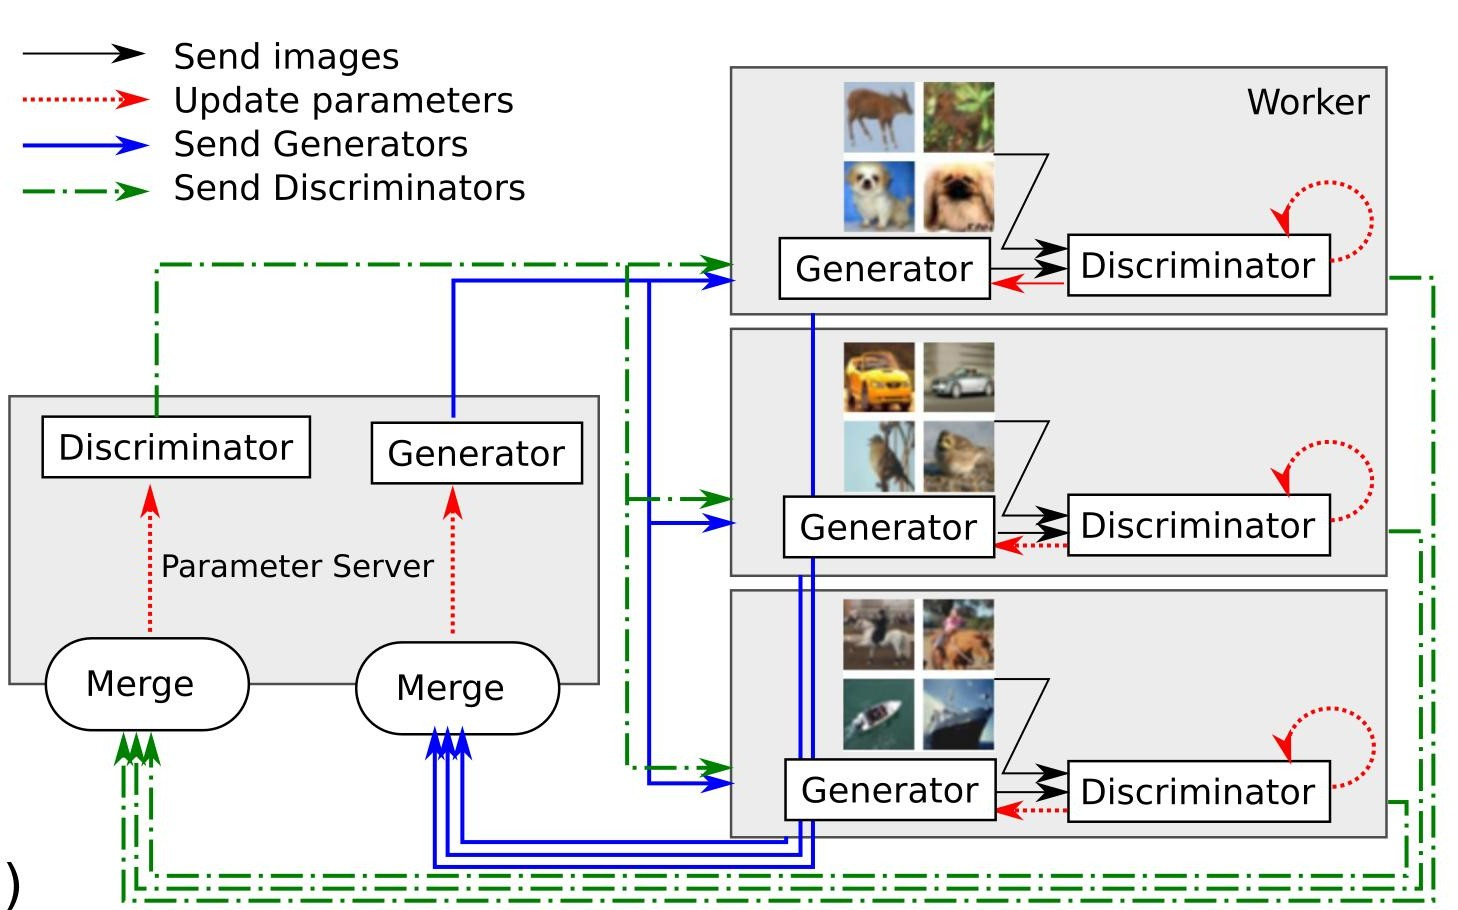
\includegraphics[width=0.49\textwidth]{./images/img3.jpeg}

\caption{FL-GAN (federated learning adapted to GAN)}

\end{figure}

\end{center}
 

\subsubsection{Experiment}

As we can see in Fig. 3 \cite{corentin2018gan}, a centralised GAN co-ordinates the workers to synchronize information and parameters. Each worker node has its own set of generator and discriminator, which train individually over different datasets, or different parts of the same dataset, and the aggregated results are sent back to the centralized generator, which will approximate and produce optimized adversarial perturbations for all the workers. The workers will be only concerned with recalculating the parameters for the localized generators, and their errors. To avoid overfitting, only a specific number of iterations over a batch will be allowed. These information on error and parameters are then relayed back to the central GAN, which then trains its own generator through its discriminator based on the data received.

The discriminators can each be individually trained over different black-box IDS models, or to attack the same black-box IDS model in a distributed manner. The output of each individual black-box at each worker will then be passed to the discriminator so that it can be emulated. The local generator will then train itself on a small batch of data, based on the output of its discriminator. This will help the distributed IDSGAN to be able to attack a distributed cluster of heterogeneous devices, in case each utilizes IDSs based on different learning models. The advantage here is that any kind of black-box can be plugged in and evaded by this model. Also, the attacking worker may be made to train on a black-box not present in that location. In this way, the actual attack location may be masked and make it difficult to track.

\subsection {Challenges}

Some of the potential challenges and problems of the above-mentioned improvements are as follows:

\begin{itemize}

\item Huge latency over a low-bandwidth network will cause the distributed IDSGAN to take a lot of time to train and generate adversarial network traffic as a lot of data will be transferred to and from workers and the central GAN.

\item If any worker is unavailable at any point of time, it will affect the training and generation of adversarial data, and may fail evasion for the black-box which the unavailable worker was targeting.

\end{itemize}

\subsection {Future work and conclusion}
Future applications for the distributed IDSGAN can be in IoT settings, where instead of a large-scale distribution, the IDSGAN will work in a relatively localized environment. Distributed IDSGAN can have applications in evading intrusion detection in real-time traffic camera networks, autonomous car navigation and update networks, OTA (Over-the-air) networks for mobile devices, distributed cloud resources and much more.

In current trends of cloud computing and fog computing, IDSGAN will have diverse applications in distributed environments, both large-scale and localized.

\section {Conclusion}
Here we have highlighted what IDSGAN is, and how it successfully had evaded most state-of-the-art IDS systems based on popular Machine Learning models. Distributed IDSGAN can even be more powerful in evasion techniques using generated adversarial traffic data. These GANs can then be used to create actually robust intrusion detection systems.

\bibliographystyle{unsrt}
\bibliography{references.bib}

\end{document}
